%%%%%%%%%%%%%%%%%%%%%%%%%%%%%%%%%%%%%%%%%
% Full Length Professional CV
% LaTeX Template
% Version 2.0 (13/6/20)
%
% Original author:
% Sreedhar Unnikrishnakurup 
%
% Important note:
% This template requires the my_cv.cls file to be in the same directory as the .tex file. The my_cv.cls file provides the resume style used for structuring the document. THe publication.bib file is needed for adding the publication list
%
%%%%%%%%%%%%%%%%%%%%%%%%%%%%%%%%%%%%%%%%%

%----------------------------------------------------------------------------------------
%	PACKAGES AND OTHER DOCUMENT CONFIGURATIONS
%----------------------------------------------------------------------------------------

\documentclass{my_cv}% Use the custom my_cv.cls style
\begin{document}
\title{CV}
\author{Sreedhar Unnikrishnakurup}
\begin{minipage}{0.8\textwidth}
\begingroup
\let\center\flushleft
\let\endcenter\endflushleft
\maketitle
\endgroup
\end{minipage}
\begin{minipage}{0.1\textwidth}
\begin{tikzpicture}[remember picture,overlay]
\clip ($(current page text area.north east)!0.01!(current page text area.south east)!-7.4!(current page text area.north west)$)
  circle (2.1cm) node {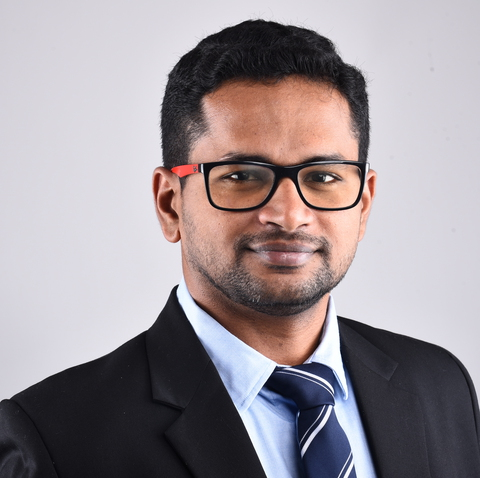
\includegraphics[width=2.3\linewidth]{mypic2}};
\end{tikzpicture}
%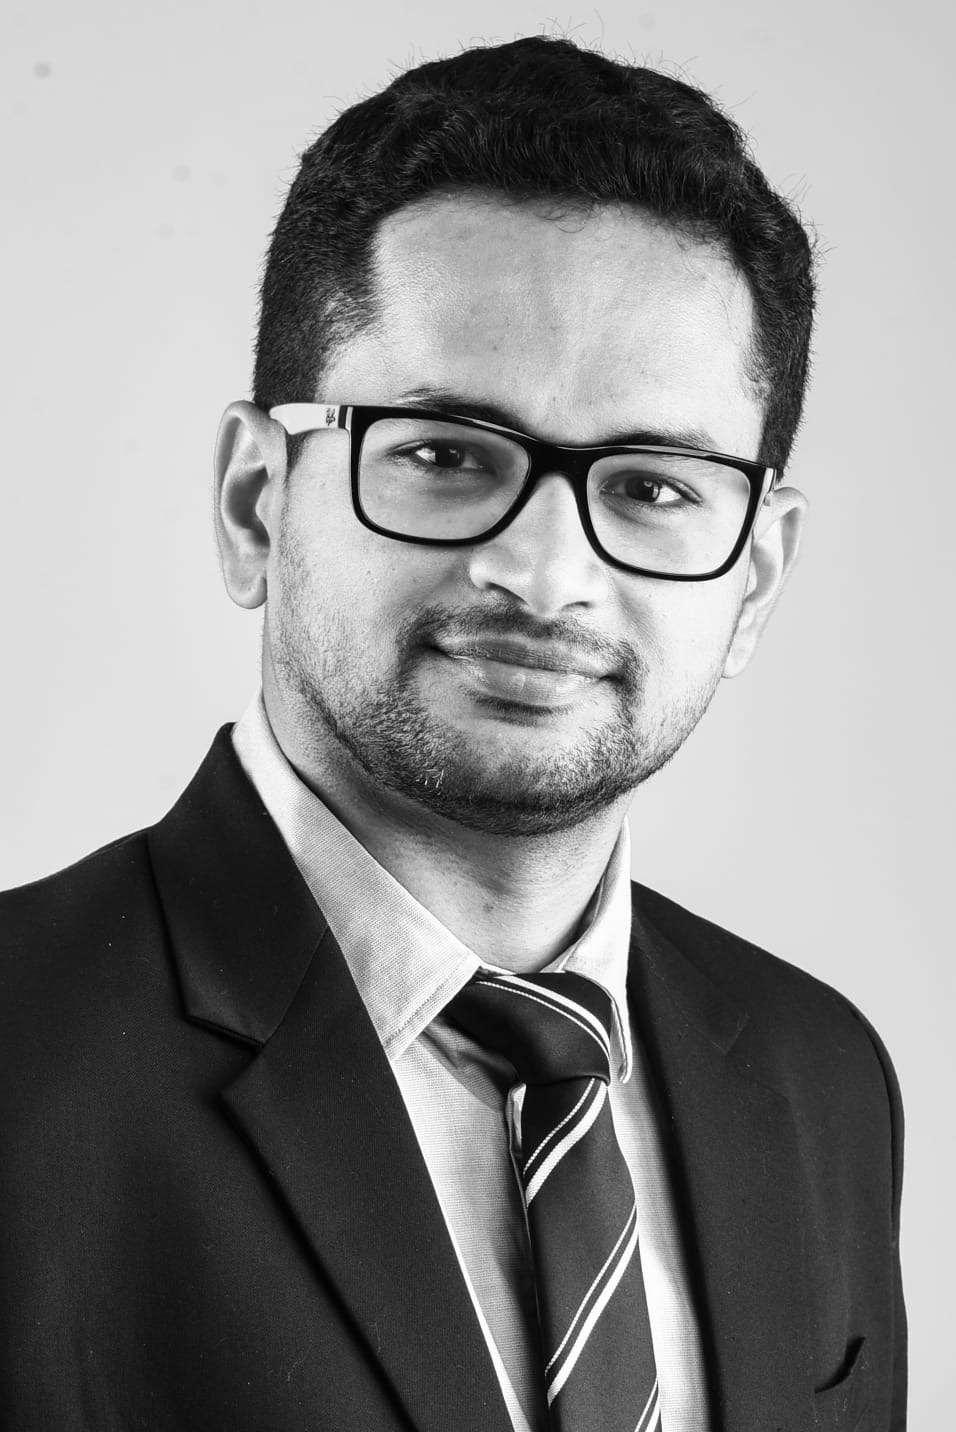
\includegraphics[width=8em]{mypic}
\end{minipage}
\vspace{1.5em}
%-------------------------------------------------------------
%	HIGHLIGHTS
%-------------------------------------------------------------
\section{Highlights}
\vspace{1.0em}
\begin{itemize}[leftmargin=0.15in]
\setlength\itemsep{-0.1em}
%\color{mygray}
\item Successfully led and secured \textbf{competitive research funding} as PI and Co-PI, including a multinational grant on curved composite inspection and a collaborative aerospace composite repair project under national R\&D programs.
\item Lead researcher for the Infrared Thermography work package in a major national polymer matrix composites programme, and a key contributor to several industry-aligned NDT projects, including early work on composite wind turbine blade inspection.
\item Published \textbf{18+ journal and 37 conference papers} in leading outlets focused on thermographic inspection of composites, demonstrating impact in the field of NDT of structural materials; additionally, filed \textbf{9 technology disclosures}, with one licensed to industry partners for practical implementation.
\item Over \textbf{10 years} of post-PhD experience in advanced NDT, with expertise in Infrared Thermography (Pulsed, Lock-in, Induction, and Laser-based IRT), as well as hands-on work with X-ray radiography, THz imaging, and ultrasonic inspection.
\item Currently \textbf{leading} the Infrared Thermography team of the Structural NDT Group at IMRE, Singapore; previously led the IRT activities at the Center for NDE, IIT Madras, as Project Officer.
\item Extensive experimental experience with sensor technologies, especially high-speed infrared cameras, and advanced NDT instrumentation for in-situ and lab-based inspection. \textbf{Level 1 certification} in Infrared Thermography.
\item Integrated machine learning into thermographic signal processing for defect detection; currently developing a multi-sensor inline inspection platform as a precursor to digital twin frameworks in composite prepreg manufacturing.
\item Proven ability to collaborate with multidisciplinary teams across academia and industry, with research experience spanning Europe and Asia.
\end{itemize}

%-------------------------------------------------------------
%	WORK EXPERIENCE SECTION
%-------------------------------------------------------------
\section{Work Experience}
\vspace{1.0em}
\subsection{Senior Scientist}
\subsubsection{\href{https://www.a-star.edu.sg/imre}{Institute of Materials Research and Engineering (IMRE), A*STAR}}
\datedsubsection{Nov 2021--Ongoing}{Singapore}
%\paragraph{
\definecolor{mypink}{rgb}{0.86, 0.08, 0.24} % Define a pink color
\hypersetup{
    colorlinks=true, % Enables colored links
    linkcolor=mypink, % Makes references (hyperref) pink
    urlcolor=blue,   % Keeps URLs in blue
    citecolor=black  % Keeps citations black
}
\begin{itemize}[leftmargin=0.15in]
\setlength\itemsep{-0.1em}
\color{mygray}
\item Project \href{https://www.a-star.edu.sg/imre/news-and-highlights/highlights/media/polymer-matrix-composites-programme-(pmcp)}{Polymer Matrix Composites Programme (PMCP)}: Managed Work Package that involved- In-line IRT monitoring of prepreg manufacturing, Characterization of damages CFRP [\textcolor{mypink}{\hyperref[J5]{J5}}, \textcolor{mypink}{\hyperref[C1]{C1}}, \textcolor{mypink}{\hyperref[C9]{C9}}], Inspection of filament wound GFRP pipes, Impact damage characterization in CFRP using Induction IRT.
\item \href{https://www.a-star.edu.sg/aerospace}{Singapore Aerospace Program} (Co-PI): UD-CFRP cross-ply laminate characterization using Induction Thermography for the composite repair [\textcolor{mypink}{\hyperref[J1]{J1}}, \textcolor{mypink}{\hyperref[J4]{J4}}, \textcolor{mypink}{\hyperref[C3]{C3}}]
\item Material Informed Differential Generative AI (\href{https://aisingapore.org/design-beyond-what-you-know-material-informed-differential-generative-ai-midgai-for-light-weight-high-entropy-alloys-and-multi-functional-composites/}{MIDGAI}) for Multi functional Composites (Project member): Development of high strength and high conductive composite using generative AI
\item Other Major projects as lead researcher: NDT evaluation using IRT and Shearography of lightning strike damage in CFRP with different Lightning strike protection materials, Water ingress detection in honeycomb sandwhich aircraft structures, Evaluation of coating porosity [\textcolor{mypink}{\hyperref[J3]{J3}}], crack detection in metallic components even under paintings using induction IRT, modeling and simulation of IRT techniques and use of AI for better defect detection [\textcolor{mypink}{\hyperref[J2]{J2}}]
\end{itemize}%}
{\color{mygray1} \hdashrule[0.1ex]{18.8cm}{0.2mm}{1mm}}
%------------------------------------------------------------
\subsection{Senior Project Officer}
\subsubsection{\href{https://www.cnde.in/}{Centre for Non-Destructive Evaluation (CNDE), IIT Madras}}
\datedsubsection{May 2018 - Sep 2021}{Chennai, India}
%\paragraph{
\begin{itemize}[leftmargin=0.15in]
\setlength\itemsep{-0.1em}
\color{mygray}
\item Application of Nondestructive IRT testing for thickness inspection of thermal barrier coatings and validation using THz-TDS and Eddy current testing [\textcolor{mypink}{\hyperref[J10]{J10}}].
\item Composite inspection using induction heating IRT. [\textcolor{mypink}{\hyperref[J7]{J7}}]
\item Crack inspection in steel billets at elevated temperatures using Laser assisted IRT [\textcolor{mypink}{\hyperref[J12]{J12}}].
\item Development of artificial intelligence-assisted advanced X-ray radiography imaging and automatic defect recognition of critical welds and high-energy materials [\textcolor{mypink}{\hyperref[J8]{J8}}]
\item Numerical investigation of anisotropic heat diffusion in polycrystalline and composite microstructures [\textcolor{mypink}{\hyperref[J11]{J11}}].
\end{itemize}%}
{\color{mygray1} \hdashrule[0.1ex]{18.8cm}{0.2mm}{1mm}}
%{\color{mygray} \rule{\linewidth}{0.5mm} }
%-----------------------------------------------------------------
\subsection{Cohort Member BA3}
\subsubsection{\href{https://www.joinef.com/}{Entrepreneur First}}
\datedsubsection{February 2020 - May 2020}{Bangalore, India}
\begin{itemize}[leftmargin=0.15in]
\setlength\itemsep{-0.1em}
\color{mygray}
\item Explored several interesting technological solutions, exploring the market, validating the technology, speaking to customers, and researching prototypes
\item The ideas that we worked on is, detect and report quality-compromised and counterfeit drugs using a mobile cloud-based cost-effective hyper-spectral Imaging based AI device
\end{itemize}
{\color{mygray1} \hdashrule[0.1ex]{18.8cm}{0.2mm}{1mm}}
%------------------------------------------------------------------
\subsection{Postdoctoral Research Scientist}
\subsubsection{\href{https://www.bam.de/Navigation/DE/Home/home.html}{NDT group 8.7, Federal Institute for Material Research and Testing (BAM)}}
\datedsubsection{January 2016 - June 2017}{Berlin, Germany}
\begin{itemize}[leftmargin=0.15in]
\setlength\itemsep{-0.1em}
\color{mygray}
\item Project \href{http://projects.npl.co.uk/vitcea/}{VITCEA} (Validated Inspection Techniques for Composites in Energy Applications) 
\item Optimize and validate active thermography as full-field, fast and non-contact NDE technique for quantitative testing of FRP structures [\textcolor{mypink}{\hyperref[J14]{J14}}]
\item Laser Thermography for surface crack detection at high temperature [\textcolor{mypink}{\hyperref[C20]{C20}}]
\end{itemize}
{\color{mygray1} \hdashrule[0.1ex]{18.8cm}{0.2mm}{1mm}}
%-----------------------------------------------------------------------
\subsection{Visiting Research Scientist}
\subsubsection{\href{https://innowacje.zut.edu.pl/cooperationoffer/electromagnetic-methods-non-destructive-testing}{Electromagnetic NDT Research Group, West Pomeranian University (ZUT)}}
\datedsubsection{January 2015 - March 2015}{Szczecin, Poland}
\begin{itemize}[leftmargin=0.15in]
\setlength\itemsep{-0.1em}
\color{mygray}
\item Scientific Exchange as part of \href{https://cordis.europa.eu/project/id/269202/results}{FP7 Project: Health Monitoring of Offshore Wind Farms (HEMOW)}
\item Terahertz imaging and time domain analysis for material defect identification in Composite Wind turbine blades [\textcolor{mypink}{\hyperref[C30]{C30}}]
\item Active Infrared Thermography for defect identification in composite materials - Numerical investigations of heat sink effects in the infrared inspecton of composites [\textcolor{mypink}{\hyperref[C26]{C26}}, \textcolor{mypink}{\hyperref[C31]{C31}}]
\end{itemize}
{\color{mygray1} \hdashrule[0.1ex]{18.8cm}{0.2mm}{1mm}}
%------------------------------------------------------------------------
\subsection{Institute Postdoctoral Fellow}
\subsubsection{\href{https://www.cnde.in/}{Centre for Non-Destructive Evaluation (CNDE), IIT Madras}}
\datedsubsection{September 2014 - December 2015}{Chennai, India}
\begin{itemize}[leftmargin=0.15in]
\setlength\itemsep{-0.1em}
\color{mygray}
\item Numerical modelling of microstructural heat diffusion and ultrasonic wave propagation in Polycrystalline Materials [\textcolor{mypink}{\hyperref[C22]{C22}}, \textcolor{mypink}{\hyperref[C24]{C24}}, \textcolor{mypink}{\hyperref[C25]{C25}}]
\item CMT welding process monitoring using IR thermography [\textcolor{mypink}{\hyperref[J16]{J16}}, \textcolor{mypink}{\hyperref[C18]{C18}}, \textcolor{mypink}{\hyperref[C21]{C21}}]
\item In-line laser thermography for Online Monitoring of steel billets to predict the surface cracks formed during the non-uniform cooling [\textcolor{mypink}{\hyperref[C23]{C23}}, \textcolor{mypink}{\hyperref[C27]{C27}}]
\end{itemize}
{\color{mygray1} \hdashrule[0.1ex]{18.8cm}{0.2mm}{1mm}}
%------------------------------------------------------------------------
\subsection{Research Associate}
\subsubsection{\href{https://www.cnde.in/}{Centre for Non-Destructive Evaluation (CNDE), IIT Madras}}
\datedsubsection{April 2007 - December 2008}{Chennai, India}
\begin{itemize}[leftmargin=0.15in]
\setlength\itemsep{-0.1em}
\color{mygray}
\item Development of online weld quality monitoring for AA2219 liquid propellant tanks using Infrared Thermal Imaging and X-ray radiography [\textcolor{mypink}{\hyperref[J18]{J18}}]
\item Developed a finite element model for the prediction of temperature profiles during welding
\end{itemize}
%-------------------------------------------------------------
%	EDUCATION SECTION
%-------------------------------------------------------------
\section{Education}
\vspace{2em}
\subsection{\href{https://adum.fr/as/ed/cv.pl?mat=39446&site=adumR} {Ph.D. in Mechanics \& Civil Engineering}}
\subsubsection{\faInstitution \hspace{0.2em} \href{https://www.umontpellier.fr/en/}{University of Montpellier 2 (UM2)}}
\datedsubsection{2011 - 2014}{Montpellier, France}
\begin{itemize}[leftmargin=0.15in]
\setlength\itemsep{-0.1em}
\color{mygray}
\item Dissertation Topic: Weld pool shape identification using Multi-physics modelling and Experiments [\textcolor{mypink}{\hyperref[D2]{D2}}, \textcolor{mypink}{\hyperref[J15]{J15}}, \textcolor{mypink}{\hyperref[C32]{C32}}-\textcolor{mypink}{\hyperref[C36]{C36}}]
\end{itemize}
{\color{mygray1} \hdashrule[0.1ex]{18.8cm}{0.2mm}{1mm}}
%-------------------------------------------------------------------------------
\subsection{M.S. in Mechanical Engineering}
\subsubsection{\faInstitution \hspace{0.2em} \href{https://www.iitm.ac.in/}{Indian Institute of Technology Madras}}
\datedsubsection{2008 - 2010}{Chennai, India}
\begin{itemize}[leftmargin=0.15in]
\setlength\itemsep{-0.1em}
\color{mygray}
\item Dissertation Topic: Online weld quality monitoring using Infrared Thermal Imaging [\textcolor{mypink}{\hyperref[D1]{D1}}, \textcolor{mypink}{\hyperref[J17]{J17}}, \textcolor{mypink}{\hyperref[J18]{J18}}, \textcolor{mypink}{\hyperref[C29]{C29}}, \textcolor{mypink}{\hyperref[C37]{C37}}]
\item Cumulative Grade Point Average 8 out of 10
\end{itemize}
{\color{mygray1} \hdashrule[0.1ex]{18.8cm}{0.2mm}{1mm}}
%--------------------------------------------------------------------------------
\subsection{Bachelors in Mechanical Engineering}
\subsubsection{\faInstitution \hspace{0.2em} \href{https://www.ieindia.org/webui/iei-home.aspx}{Institution of Engineers India}}
\datedsubsection{2002 - 2006}{Kottayam, India}
\begin{itemize}[leftmargin=0.15in]
\setlength\itemsep{-0.1em}
\color{mygray}
\item Cumulative Grade Point Average 6.94 out of 10
\end{itemize}
%-------------------------------------------------------------
%	Publication
%-------------------------------------------------------------
\section{Publication}
\vspace{1em}
\nobibliography{publication}
%\bibliographystyle{unsrt}
\begin{comment}
\begin{itemize}
    \item 16 Journal publication and 12 conference presentations.
    \item Complete list of publication is available at URL: \href{https://bit.ly/30BlL05}{https://bit.ly/30BlL05}
\end{itemize}
\end{comment}
 \bibliographystyle{unsrtnat}
\subsection{\faBook \hspace{0.2em} \bfseries Dissertations}
\vspace{1em}
\renewcommand{\theenumi}{D\arabic{enumi}}
\begin{enumerate}
\setlength\itemsep{-0.1em}
\color{mygray}
 \item \bibentry{sreedhar2014} 
 \item \bibentry{sreedhar2011} 
\end{enumerate}

\subsection{\faFileTextO \hspace{0.5em}\bfseries Journal Articles}
\vspace{1em}
\renewcommand{\theenumi}{J\arabic{enumi}} % Change numbering format to J1, J2, ...
\begin{enumerate}
\setlength\itemsep{-0.1em}
%\setlength\itemsep{-0.1em}
\color{mygray}
 \item \label{J1} \bibentry{unnikrishnakurup2025assessment} 
 \item \label{J2} \bibentry{bounenni2024advanced} 
 \item \label{J3} \bibentry{unnikrishnakurup2024exploring} 
 \item \label{J4} \bibentry{kidangan2024uncovering} 
 \item \label{J5} \bibentry{kidangan2024induction} 
 \item \label{J6} \bibentry{Mercy2022} 
 \item \label{J7} \bibentry{Renil2022} 
 \item \label{J8} \bibentry{Dhruv2021} 
 \item \label{J9} \bibentry{Surendra2021} 
 \item \label{J10} \bibentry{Sreedhar2020} 
 \item \label{J11} \bibentry{Saini2020} 
 \item \label{J12} \bibentry{puthiyaveettil2020} 
 \item \label{J13} \bibentry{Nithin2019} 
 \item \label{J14} \bibentry{maierhofer2018} 
 \item \label{J15} \bibentry{unnikrishnakurup2017} 
 \item \label{J16} \bibentry{thomas2017} 
 \item \label{J17} \bibentry{sreedhar2016} 
 \item \label{J18} \bibentry{sreedhar2012} 
\end{enumerate}

\begin{comment}
\subsection{\faFileTextO \hspace{0.5em}\bfseries Forthcoming [Under Review]}
\vspace{1em}
\begin{enumerate}
\setlength\itemsep{-0.1em}
\color{mygray}
 \item\bibentry{Renil2023} \cite{Renil2023}
\end{enumerate}
\end{comment}

\subsection{\faFilePowerpointO \hspace{0.5em}\bfseries Conference Presentations}
\renewcommand{\theenumi}{C\arabic{enumi}} % Change numbering format to C1, C2, ...
\begin{enumerate}
\setlength\itemsep{-0.1em}
\color{mygray}
\item \label{C1} \bibentry{unnikrishnakurup2025lockin}
\item \label{C2} \bibentry{zheng2024multispectral}
\item \label{C3} \bibentry{unnikrishnakurup2023characterizing}
\item \label{C4} \bibentry{gnessougoucurved}
\item \label{C5} \bibentry{unnikrishnakurup1exploring}
\item \label{C6} \bibentry{kumara2022dynamic}
\item \label{C7} \bibentry{zheng2022using}
\item \label{C8} \bibentry{unnikrishnakurup2022crack} 
\item \label{C9} \bibentry{Sreeconf2022} 
\item \label{C10} \bibentry{Jyoticonf2020} 
\item \label{C11} \bibentry{Surendraconf2020} 
\item \label{C12} \bibentry{Dhruv2019} 
\item \label{C13} \bibentry{Sreedharconf2020} 
\item \label{C14} \bibentry{Sruthiconf2018} 
\item \label{C15} \bibentry{Nithinconf2018} 
\item \label{C16} \bibentry{Maierhoferconf2018} 
\item \label{C17} \bibentry{Krishnaconf2017} 
\item \label{C18} \bibentry{Renilconf2016} 
\item \label{C19} \bibentry{Nithinconf2016} 
\item \label{C20} \bibentry{Polomskiconf2016} 
\item \label{C21} \bibentry{Kidanganconf2016} 
\item \label{C22} \bibentry{Shivaprasadconf2015} 
\item \label{C23} \bibentry{Sreedharconf2015} 
\item \label{C24} \bibentry{Shivaprasadcomsolconf2015} 
\item \label{C25} \bibentry{SreedharQIRTconf2015} 
\item \label{C26} \bibentry{SzymznikQIRTconf2015} 
\item \label{C27} \bibentry{SreeQIRTconf2015} 
\item \label{C28} \bibentry{SreeSGRconf2015} 
\item \label{C29} \bibentry{SreePolandconf2015} 
\item \label{C30} \bibentry{Chadyconf2015} 
\item \label{C31} \bibentry{Barbaraconf2014} 
\item \label{C32} \bibentry{Rouquetteconf2014} 
\item \label{C33} \bibentry{Sreedharconf2013} 
\item \label{C34} \bibentry{Sreedharconf2012} 
\item \label{C35} \bibentry{SreedharNconf2012} 
\item \label{C36} \bibentry{Rouquetteconf2011} 
\item \label{C37} \bibentry{Sreedharconf2009} 
\end{enumerate}
%\end{comment}
\subsection{\faLightbulbO \hspace{0.5em}\bfseries Innovation and Technology Transfer}

\begin{itemize}
\setlength\itemsep{-0.1em}
  \item Filed \textbf{9 Technology Disclosures} at Institute of Materials Research and Engineering (IMRE), A*STAR between 2021–2025 in the areas of Infrared Thermography, Composite Inspection, and Laser-Based NDT.
  \item \textbf{1 TD licensed} to industry partner for use in  composite inspection workflows in bicycle repair.
\end{itemize}

%-------------------------------------------------------------
%	             INVITED PRESENTATION
%-------------------------------------------------------------
\begin{comment}
\section{Invited Presentations}
\vspace{1em}
\begin{itemize}[leftmargin=0.15in]
\setlength\itemsep{-0.1em}
\color{mygray}
\item Preconference Tutorials, NDE 2019 Organized by Indian Society for Non-Destructive Evaluation ISNT, Talk: Applications of thermal imaging in aerospace industry, Bengaluru, December 3, 2019
\item Workshop on Advanced NDE Techniques and Applications organized by TATA STEEL, Talk: Advanced Thermography Techniques, TATA Nagar, Jamshedpur, India, August 17, 2015
\item Polish society for theoretical and applied electrical engineering section in Szczecin (PTETiS), Talk: Research and Development in the field of NDE @ CNDE, West Pomeranian University of Technology, Szczecin, Poland, March 12, 2015
\item Polish society for nondestructive testing and technical diagnostic section in Szczecin (PTBNiDT), Talk: Research and Applications of IR Thermography @ CNDE, Szczecin, Poland, February 26, 2015
\end{itemize}
\end{comment}
%--------------------------------------------------------------
%	              RESEARCH INTEREST
%-------------------------------------------------------------
\begin{comment}
\section{Research Interest}
\vspace{1em}
\begin{itemize}[leftmargin=0.15in]
\setlength\itemsep{-0.1em}
\color{mygray}
\item Developing signal processing algorithms for acoustic, seismic, or electromagnetic data
\item Applying machine learning techniques to signal processing problems
\item Analyzing data from different sources and extract meaningful insights
\item Developing new signal processing techniques for challenging environments

\end{itemize}
\end{comment}
%---------------------------------------------------------------
%	                 SKILLS SECTION
%-------------------------------------------------------------
\section{Skills}
\vspace{1em}
\begin{minipage}{0.35\textwidth}
\cvSkill{5}    MATLAB \\           
\cvSkill{4}  Python \\
   
\end{minipage}
\begin{minipage}{0.35\textwidth}
\cvSkill{5}   FEM: COMSOL \\
\cvSkill{4}   \LaTeX \\

\end{minipage}
\begin{minipage}{0.35\textwidth}
\cvSkill{5}   Deep learning \\
\cvSkill{4}   Machine Learning \\

\end{minipage}
%--------------------------------------------------------------
%	                 Grants and Fellowships
%-------------------------------------------------------------
\begin{comment}
\section{Grants and Fellowships}
\vspace{1em}
\grantsubsection{Travel Grant to attend international scientific event from Council of Scientific \& industrial Research }{2019}
\grantsubsection{Visiting Researcher Fellowship under EU Project  Health Monitoring of Offshore Wind Farms (HEMOW)}{2015}
\grantsubsection{Institute Postdoctoral Research Grant from Indian Institute of Technology Madras}{2014-2015}
\grantsubsection{French research allowance from University of Montpellier for carrying out Ph.D.}{2011-2013}
\grantsubsection{Post-Graduate Fellowship: GATE from Govt. of India}{2008-2010}
\end{comment}
%-------------------------------------------------------------
%	                 Certifications and Courses
%-------------------------------------------------------------
\section{Certifications and Memberships}
\vspace{1em}
\begin{itemize}[leftmargin=0.15in]
\setlength\itemsep{-0.1em}
\color{mygray}
\item[\faCertificate] Project Management Fundamentals by EPM Issued on October 2022
\item[\faCertificate] Infrared Thermography Level 1 by Infrared Training Center. Issued on May 2022
\item[\faCertificate] Deep Learning, a 5-course specialization by deeplearning.ai on Coursera. Specialization Certificate earned on September 23, 2018
\item [\faUsers] QIRT ASIA Steering committe Member
\item [\faUsers] Member of Indian Society for Nondestructive Evaluation
\item [\faUsers] Member of Institution of Engineers (India), and Chartered Engineer Certification
\item [\faUsers] Member of NonDestructive Testing Society Singapore (NDTSS)
%\item[\faCertificate] Fundamentals of Data Science \& Deep learning course, PadhAI, One fourth labs, IIT Madras (Ongoing, July 2020)
\end{itemize}

%-------------------------------------------------------------
%	                 Languages
%-------------------------------------------------------------
\section{Languages}
\vspace{1em}
\noindent
\begin{minipage}{0.4\textwidth}
\begin{itemize}
\setlength\itemsep{0.0em}
\item[] English  \hspace{0.5em} \cvSkill{5} 
\item[] German  \hspace{0.2em} \cvSkill{3} 
\item[] French  \hspace{0.8em} \cvSkill{2}
\end{itemize}
\end{minipage}
%second column
\begin{minipage}{0.4\textwidth}
\begin{itemize}
\setlength\itemsep{0.0em}
\item[] Malayalam  \hspace{0.5em} \cvSkill{5} 
\item[] Hindi      \hspace{2.9em} \cvSkill{4} 
\item[] Tamil      \hspace{2.9em} \cvSkill{3}
\end{itemize}
\end{minipage}
\vspace{2em}
%----------------------------------------------------------------
%	Mentoring Activities
%----------------------------------------------------------------
%\begin{comment}
\section{Mentoring}
\vspace{1em}
\noindent \faEye \hspace{1em} \color{mygray} During postdoctoral tenure at IIT Madras: 4 Ph.D. Students and 2 Master student 
\begin{itemize}[leftmargin=0.15in]
\setlength\itemsep{-0.1em}
\color{mygray}
\item Shivaprasad S (Ph.D.) - Voronoi Cell based FEM simulations for wave propagation in solids [\textcolor{mypink}{\hyperref[C22]{C22}}, \textcolor{mypink}{\hyperref[C24]{C24}}]
\item Renil Thomas K (Ph.D.) - Induction thermography inspection of CFRP and CMT weld monitoring [\textcolor{mypink}{\hyperref[J1]{J1}}, \textcolor{mypink}{\hyperref[J4]{J4}}, \textcolor{mypink}{\hyperref[J7]{J7}}, \textcolor{mypink}{\hyperref[J16]{J16}}] 
\item Nithin P V (Ph.D.) - Laser thermography for carack inspection in steel samples at elevated temperature [\textcolor{mypink}{\hyperref[J12]{J12}}, \textcolor{mypink}{\hyperref[J13]{J13}}]
\item Surendra Gupta (Ph.D.) - Emissivity characterization of nano photonic emitters [\textcolor{mypink}{\hyperref[J9]{J9}}]
\item Anurag Saini (MTech) - Numerical investigation of Heat diffusion in particle reinforced composite [\textcolor{mypink}{\hyperref[J11]{J11}}]
\item Dhruv Gamdha (MTech) - Ray tracing model for X-ray simulation and AI based automatic defect Recognition [\textcolor{mypink}{\hyperref[J8]{J8}}]
\end{itemize}
%\end{comment}
%---------------------------------------------------------------
%	Reference
%----------------------------------------------------------------
\section{References}
\vspace{1em}
\begin{minipage}{0.6\textwidth}
\subsubsection{Prof. Krishnan Balasubramaniam} 
\faAt \hspace{0.2em} \href{mailto:balas@iitm.ac.in}{balas@iitm.ac.in} \\
\hspace{0.5em} \faInstitution \hspace{0.2em} \href{http://iitm.irins.org/profile/50968}{Department of Mechanical Engineering, IIT Madras}
\vspace{1.5em}
\subsubsection{Dr. Fabien Soulie} 
\faAt \hspace{0.2em} \href{mailto:fabien.soulie@umontpellier.fr}{fabien.soulie@umontpellier.fr}\\ \hspace{0.2em}\faInstitution \hspace{0.2em}  \href{http://www.lmgc.univ-montp2.fr/spip.php?page=pageperso&nom=SOULIE&prenom=Fabien&lang=fr}{UM2/LMGC}
\vspace{1em}
\end{minipage}
\begin{minipage}{0.6\textwidth}
\subsubsection{Dr. Sebastien Rouquette} 
\faAt \hspace{0.2em} \href{mailto:sebastien.rouquette@umontpellier.fr}{sebastien.rouquette@umontpellier.fr}\\ \faInstitution \hspace{0.2em} \href{http://www.lmgc.univ-montp2.fr/spip.php?page=pageperso&nom=ROUQUETTE&prenom=Sebastien&lang=fr}{UM2/LMGC}
\vspace{1.2em}
\subsubsection{Dr. C. V. Krishnamurthy} 
\faAt \hspace{0.2em} \href{mailto:cvkm@iitm.ac.in}{cvkm@iitm.ac.in} \\
\faInstitution \hspace{0.2em} \href{http://iitm.irins.org/profile/61936}{Department of Physics, IIT Madras}
\end{minipage}
%-------------------------------------------------------------
\end{document}




\begin{comment}
\subsubsection{Dr. C. V. Krishnamurthy} 
\faAt \hspace{0.2em} \href{mailto:cvkm@iitm.ac.in}{cvkm@iitm.ac.in} \\
\faInstitution \hspace{0.2em} \href{http://iitm.irins.org/profile/61936}{Department of Physics, IIT Madras}
\subsubsection{}
\vspace{4.8em}
\end{comment}